% setup the document and include packages
\documentclass{article}[12pt]
\usepackage{graphicx}
\usepackage{amsmath}
\usepackage{amssymb}
\usepackage{cancel}
\usepackage{ntheorem}
\usepackage{algorithm2e}
\usepackage{float}
\usepackage{caption}
\usepackage{fancyvrb}
\usepackage[dvipsnames]{xcolor}
\usepackage[section]{placeins}
\usepackage[toc,page]{appendix}
\usepackage{hyperref}

%set stuff for syntax highlighting
\usepackage{fontspec}
\usepackage{minted}
\setsansfont{Calibri}
\setmonofont{Consolas}


\hypersetup{
    colorlinks=true,
    linkcolor=blue,
    filecolor=magenta,      
    urlcolor=cyan,
}
\urlstyle{same}

\makeatletter
\def\BState{\State\hskip-\ALG@thistlm}
\makeatother

\makeatletter
\g@addto@macro\@floatboxreset\centering
\makeatother

% define Continue for algorithms
\SetKw{Continue}{continue}

% Define custome verbatim command to insert maze text file results
\RecustomVerbatimCommand{\BVerbatimInput}{VerbatimInput}%
{fontsize=\footnotesize,
 %
 frame=lines,  % top and bottom rule only
 framesep=2em, % separation between frame and text
 rulecolor=\color{Black},
 %
 %label=\fbox{\color{Black}data.txt},
 labelposition=topline,
 %
 %commandchars=\|\(\), % escape character and argument delimiters for
                      % commands within the verbatim
 %commentchar=*        % comment character
}

% redefine QED symbol
\renewcommand{\qedsymbol}{\rule{0.7em}{0.7em}}

% define lemma and result theorem-styled sections
\newtheorem{lemma}{Lemma}[section]
\newtheorem{result}{Result}[section]

% Don't print the semicolon in algorithms
\DontPrintSemicolon

% define the title that will be used in the report
\title{CS 598 PS \\ Machine Learning for Signal Processing \\ Problem Set 2}
\author{
Christian Howard \\ howard28@illinois.edu
}
\date{} % don't set a date because we don't need this shit


% setup paths for images
\graphicspath{ {../scripts/} }

% start the document
\begin{document}
   
   % create the title page 
   \maketitle
   \begin{abstract}
   	Within this report is a set of solutions for Problem Set 2 spanning areas of linear and nonlinear unsupervised learning applied to sound and images. In the first problem, Principle Component Analysis (PCA), Independent Component Analysis (ICA), Non-negative Matrix Factorization (NMF), and, for fun, a method being called a Randomized Projection (RP) were applied to identifying three different types of sounds played in a recording based on a spectrogram of the sound signal. The second problem used PCA, ICA, and NMF to again identify features, this time for a dataset of hand written digits. In the first two problems, it was found that NMF produced more intuitive features and weights that were purely positive and in turn additive. Additionally, ICA tended to create a much more independent looking set of features than the PCA data it was based on, as expected. In the third problem, PCA and Laplacian Eigenmaps were used to try and understand the structure of the digit 6 subset. It was found that PCA did not do a great job of showing the nonlinear structure of this data while Laplacian Eigenmaps did very well at achieving this.
   \end{abstract}
   \newpage
   
   % create table of contents on separate page
   \tableofcontents
   \newpage
   
   \section{Problem 1 - An Audio Features Project}
   Within this problem, the goal is to use a set of dimensionality reduction and feature selection techniques to find three features that can help identify three different sounds in a recording. The methods being reviewed are PCA, ICA, Non-negative Matrix Factorization (NMF), and then for fun I wrote an algorithm, call is the Randomized Projection (RP), that forms a low-rank approximation via projection form to the data $D$ using randomized algorithms such that $D = Q(Q^T D) = Q B$ and $Q^T Q = I$. Before jumping into the analysis with the various feature selection methods, Figure \ref{fig:spectro} represents a visual of the spectrogram for the input sound which will be the data set being passed into the set of algorithms.
   
   \begin{figure}[ht]
   \centerline{
   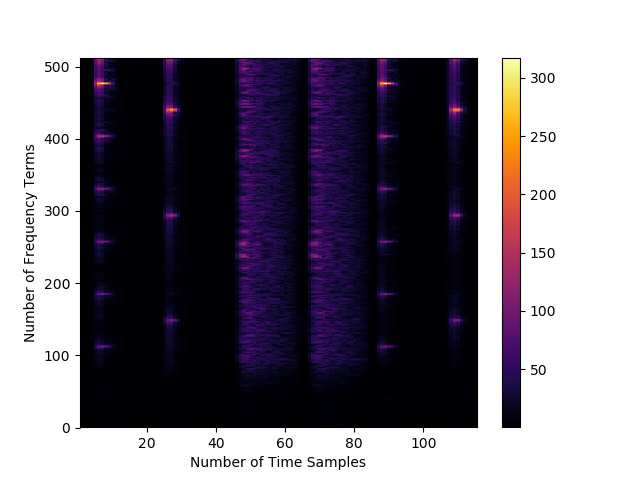
\includegraphics[scale=1.0]{p1/spectrogram.png}}
   \caption{Spectrogram of Sound}
   \label{fig:spectro}
   \end{figure}
   
   With Figure \ref{fig:spectro} representing the input data set, one can then produce the three features using each method. Figures \ref{fig:pca_f} and \ref{fig:pca_w} represent the features and weights generated by PCA. Figures \ref{fig:ica_f} and \ref{fig:ica_w} represent the features and weights generated by chaining PCA and ICA. Figures \ref{fig:nmf_f} and \ref{fig:nmf_w} represent the features and weights generated by NMF. Figures \ref{fig:rp_f} and \ref{fig:rp_w} represent the features and weights generated by the RP approach. In terms of observations, all of the methods produce features with generally similar patterns. However, ICA definitely produces features that appear more independent than those of PCA. The RP approach also produces a very similar set of features to PCA but without having to compute an expensive SVD.
   
   Additionally, PCA and ICA have features that have components that are negative and positive, while NMF has features that have purely positive components. This difference produces interesting behavior in the weights because PCA and ICA have both negative and non-negative weights, while NMF produces purely positive weights. At least for myself, NMF produces the pair of features and weights that make the most sense. This is not only because can you view the sound frequencies as purely additive, which is more intuitive, but when the weights are most positive, you can easily tell that is when a feature is most activated. For ICA and PCA, it is harder due to the mix of negative and positive weights and feature components.
  
   \begin{figure}[ht]
   \centerline{
   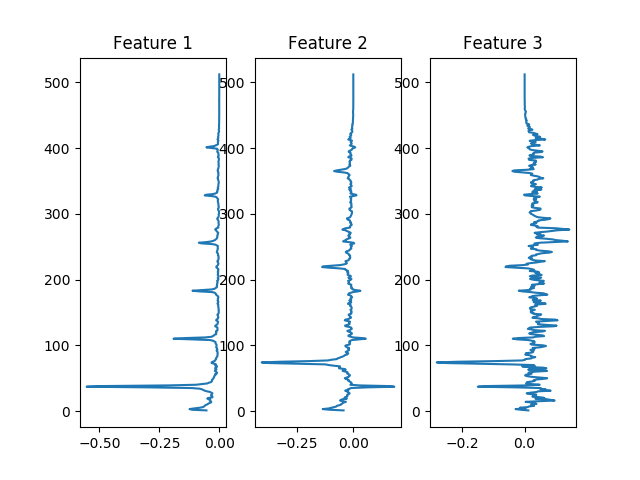
\includegraphics[scale=1.0]{p1/pca_features_sound.png}}
   \caption{PCA Features}
   \label{fig:pca_f}
   \end{figure}
   
   \begin{figure}[ht]
   \centerline{
   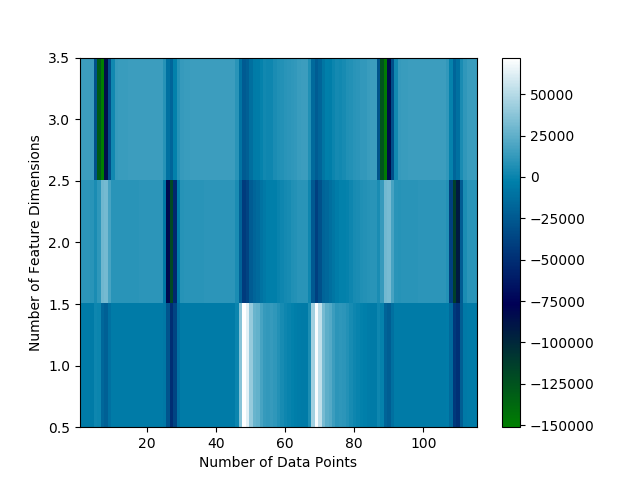
\includegraphics[scale=1.0]{p1/pca_weights_sound.png}}
   \caption{PCA Weights}
   \label{fig:pca_w}
   \end{figure}   


   \begin{figure}[ht]
   \centerline{
   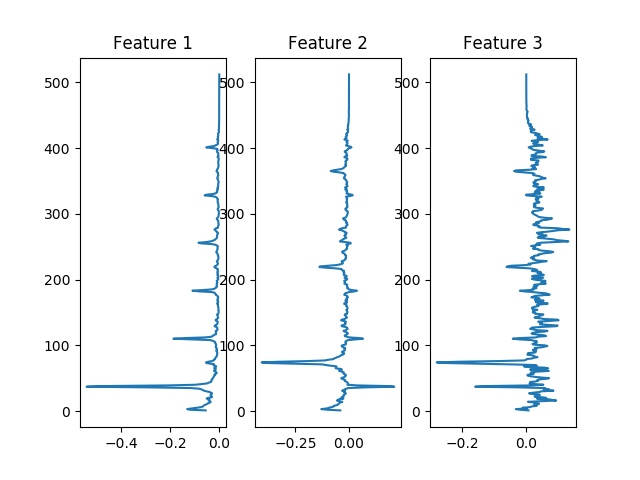
\includegraphics[scale=1.0]{p1/randproj_features_sound.png}}
   \caption{Randomized Projection Features}
   \label{fig:rp_f}
   \end{figure}
   
   \begin{figure}[ht]
   \centerline{
   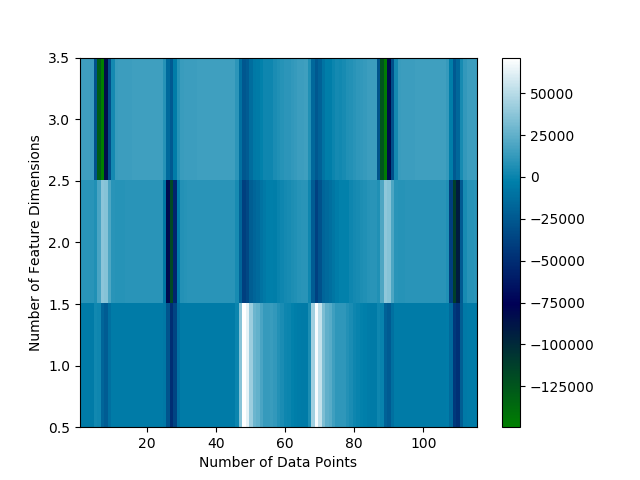
\includegraphics[scale=1.0]{p1/randproj_weights_sound.png}}
   \caption{Randomized Projection Weights}
   \label{fig:rp_w}
   \end{figure}  

   
   \begin{figure}[ht]
   \centerline{
   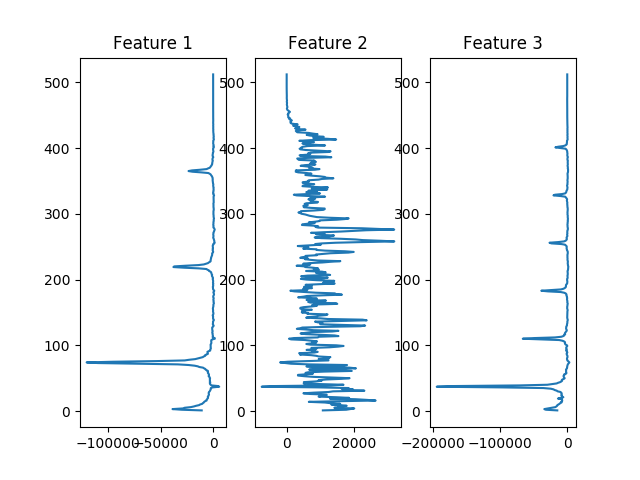
\includegraphics[scale=1.0]{p1/ica_features_sound.png}}
   \caption{ICA Features}
   \label{fig:ica_f}
   \end{figure}
   
   \begin{figure}[ht]
   \centerline{
   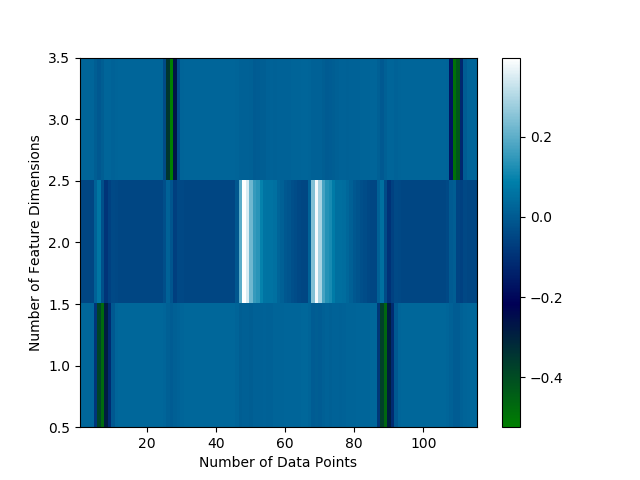
\includegraphics[scale=1.0]{p1/ica_weights_sound.png}}
   \caption{ICA Weights}
   \label{fig:ica_w}
   \end{figure}
   
   \begin{figure}[ht]
   \centerline{
   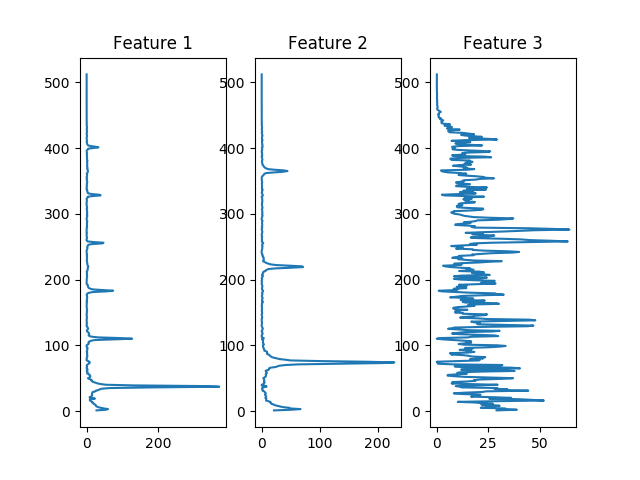
\includegraphics[scale=1.0]{p1/nmf_features_sound.png}}
   \caption{NMF Features}
   \label{fig:nmf_f}
   \end{figure}
   
   \begin{figure}[ht]
   \centerline{
   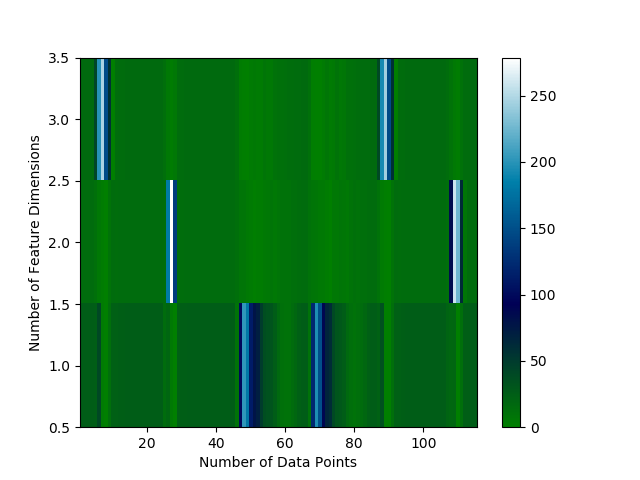
\includegraphics[scale=1.0]{p1/nmf_weights_sound.png}}
   \caption{NMF Weights}
   \label{fig:nmf_w}
   \end{figure}
   
   \newpage
   \section{Problem 2 - Handwritten Digit Features}
   Within this section, we look at finding features for a data set of hand drawn digits. In particular, we are tasked to find 36 features using PCA, ICA, and NMF. Figures \ref{fig:pca_dig_f}, \ref{fig:ica_dig_f}, and \ref{fig:nmf_dig_f} display features found using PCA, ICA, and NMF. 
   
   As in Problem 1, PCA and ICA produce features that share the trait of having components that range from being positive to negative while NMF has features with purely positive components. This difference makes NMF produce features that are very different from PCA and ICA, again allowing NMF's features to be purely additive and fairly intuitive. When comparing PCA and ICA, we can see that ICA has features that are appear more independent than that of PCA. This is because ICA's features tend to be more distinct features while PCA has features that share similarities. This is obviously expected since ICA strives to obtain independent features while PCA is just looking to create decorrelated features.
   
   \begin{figure}[ht]
   \centerline{
   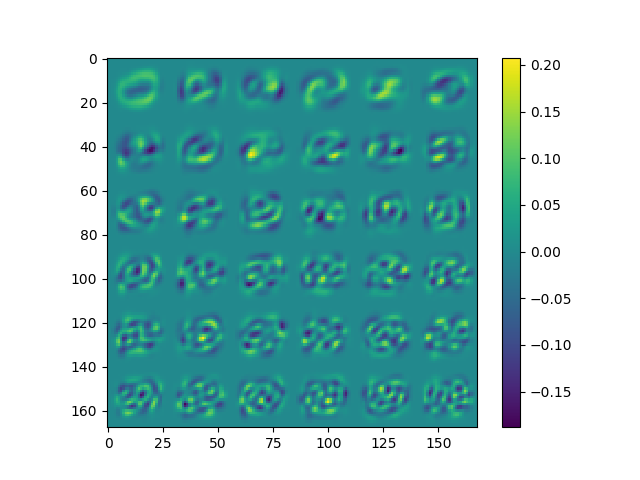
\includegraphics[scale=0.7]{p2/pca_features_digits.png}}
   \caption{PCA Digit Features}
   \label{fig:pca_dig_f}
   \end{figure}
   
   \begin{figure}[ht]
   \centerline{
   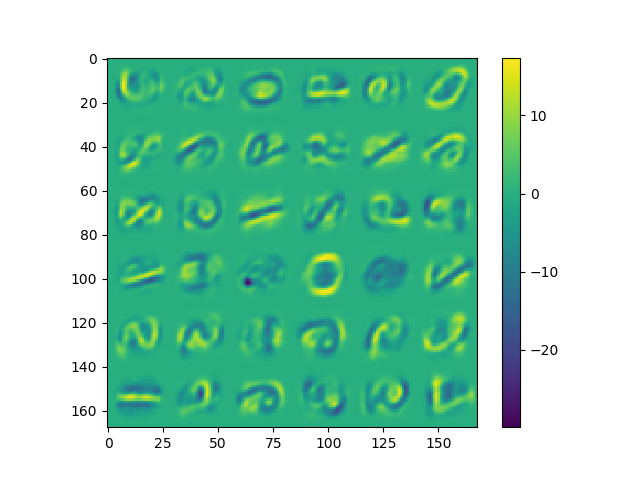
\includegraphics[scale=0.7]{p2/ica_features_digits.png}}
   \caption{ICA Digit Features}
   \label{fig:ica_dig_f}
   \end{figure}
   
   \begin{figure}[ht]
   \centerline{
   \includegraphics[scale=0.7]{p2/NMF_features_digits.png}}
   \caption{NMF Digit Features}
   \label{fig:nmf_dig_f}
   \end{figure}
   
   \newpage
   \section{Problem 3 - The Geometry of Handwritten Digits}
   Within this problem, we extend work done in Problem 2 by investigating patterns for the digit 6 in the data set. We start off this investigation by performing PCA on this subset of data to find 2 features, shown below in Figure \ref{fig:pca_f6}. 
   
   \begin{figure}[ht]
   \centerline{
   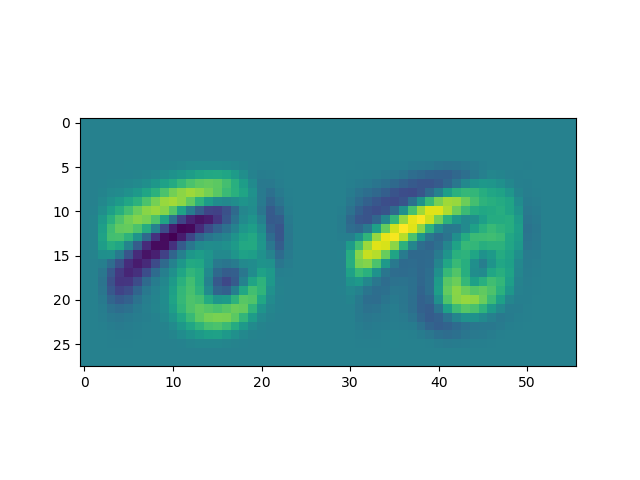
\includegraphics[scale=0.7]{p3/pca_features_6.png}}
   \caption{PCA Digit 6 Features}
   \label{fig:pca_f6}
   \end{figure}
   
   If we take weights associated with the above features, we can plot them in a 2D scatter plot with their associated image from the original data set. We can see the result of such a thing in Figure \ref{fig:pca_scatter}.
   
   \begin{figure}[ht]
   \centerline{
   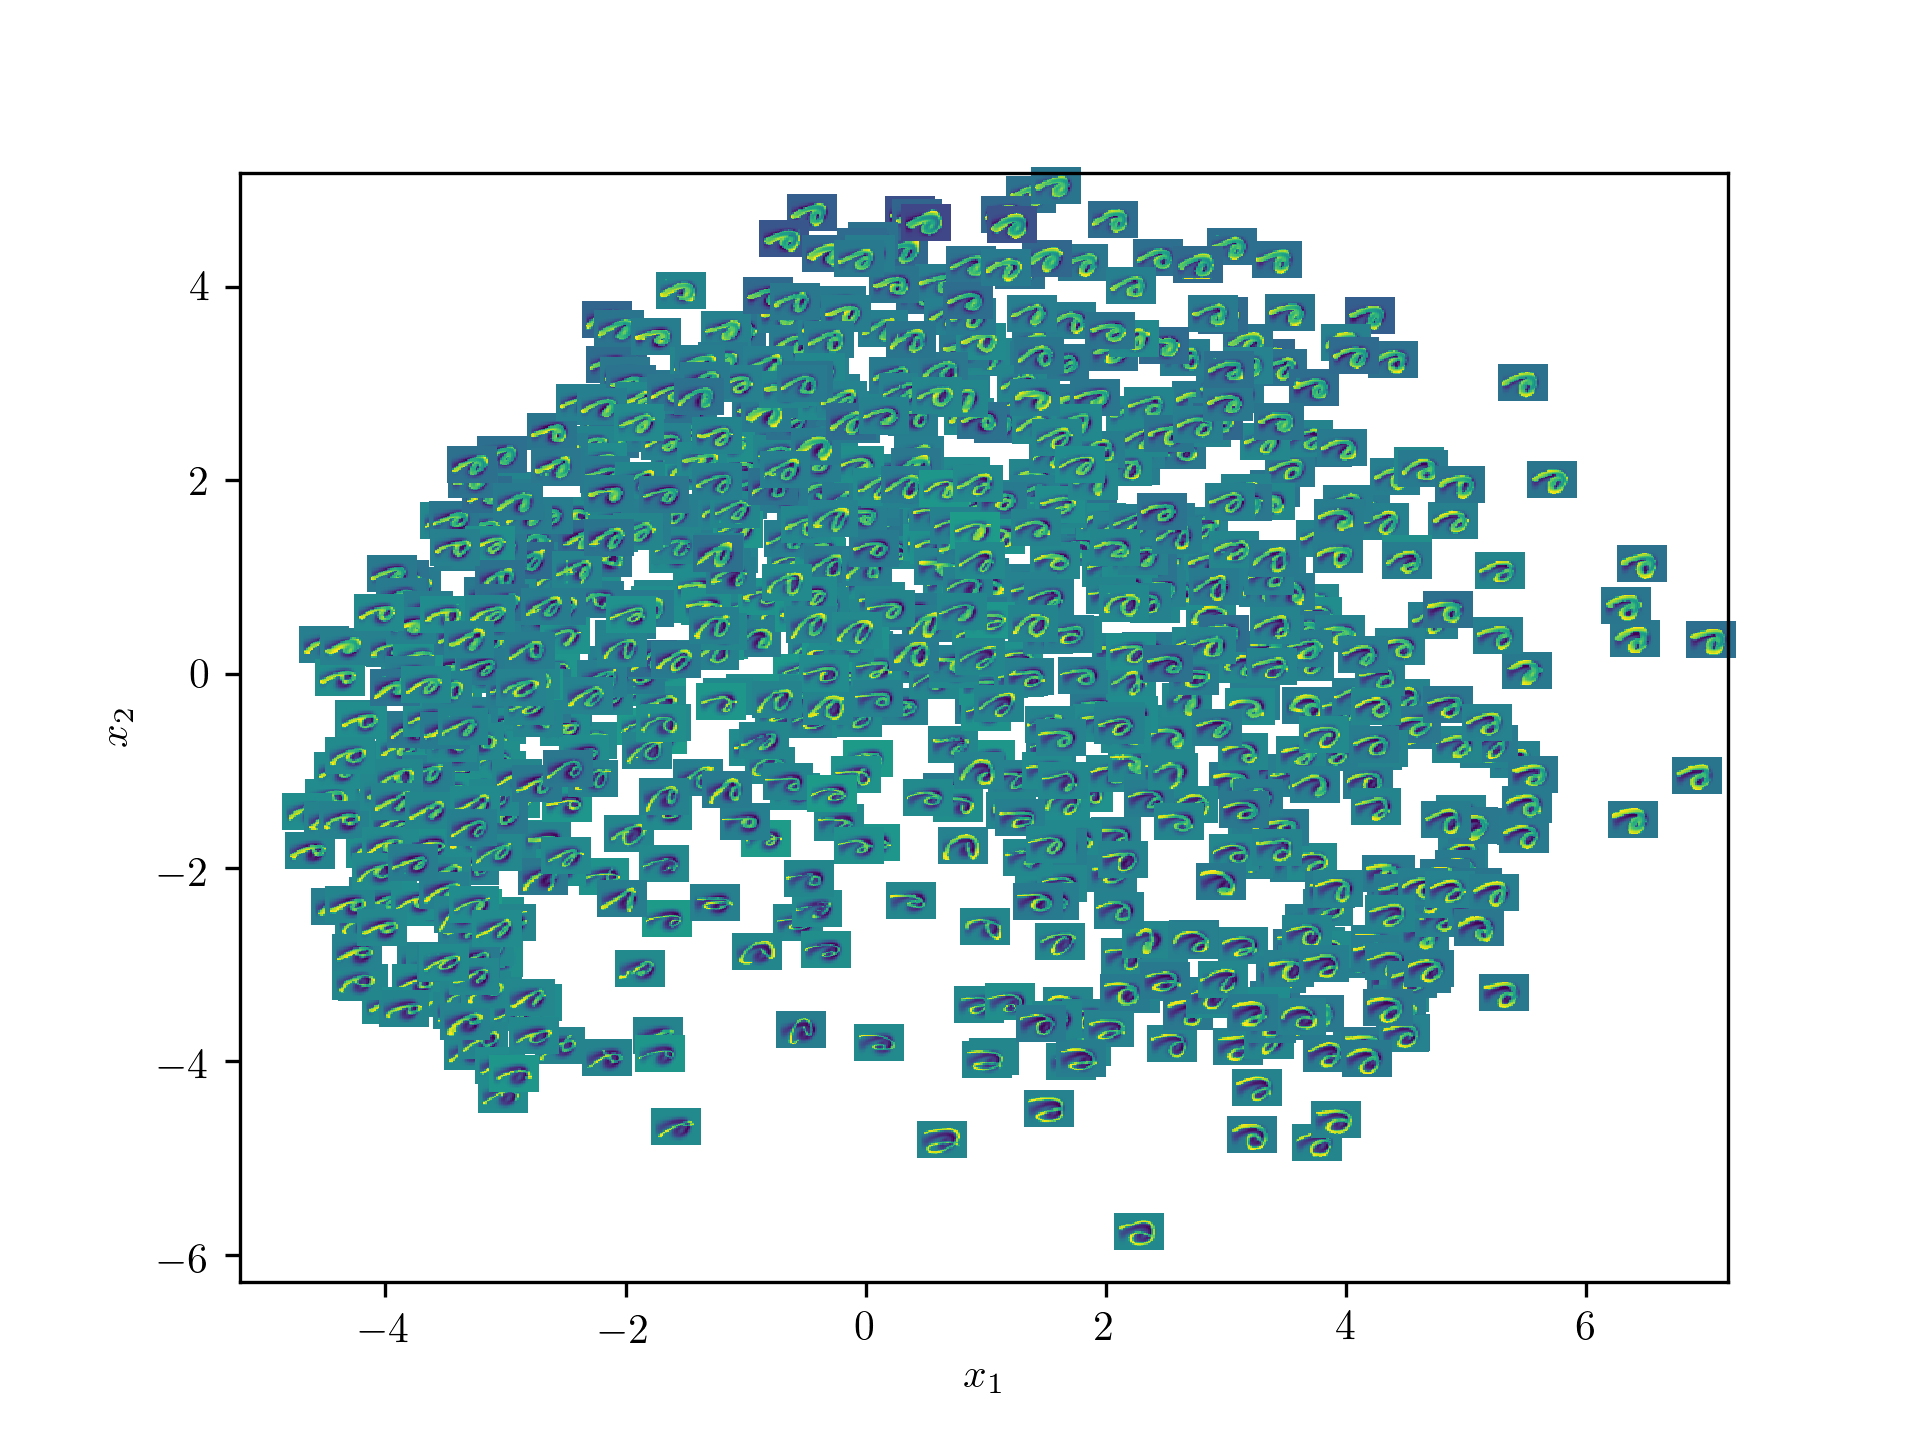
\includegraphics[scale=1.4]{p3/pca_weightspace_images_6.png}}
   \caption{PCA Weight Space Scatter Plot}
   \label{fig:pca_scatter}
   \end{figure}
   
   As we look at Figure \ref{fig:pca_scatter}, we can see there appears to be a pattern going from left to right in the similarity between images. To see if there is some structure we can identify, we can use a Spectral Embedding via a Laplacian Eigenmap to see if we can find some underlying manifold for the data. For this case, we will produce this Laplacian Eigenmap using 10 nearest neighbors and again ensure we end up with two dimensional features. Figure \ref{fig:leig_scatter} shows the resulting 2D scatter plot of the data set's images tied to their associated weight vectors. 
   
   As we can readily see as we compare Figure \ref{fig:pca_scatter} to Figure \ref{fig:leig_scatter}, there indeed appears to be some underlying nonlinear structure for the 6 digit data set that has become more apparent after the embedding. This shows there is indeed a strong, nonlinear relationship between the data for the digit 6 that has been found via the manifold the Laplacian Eigenmap estimated.
   
   \begin{figure}[ht]
   \centerline{
   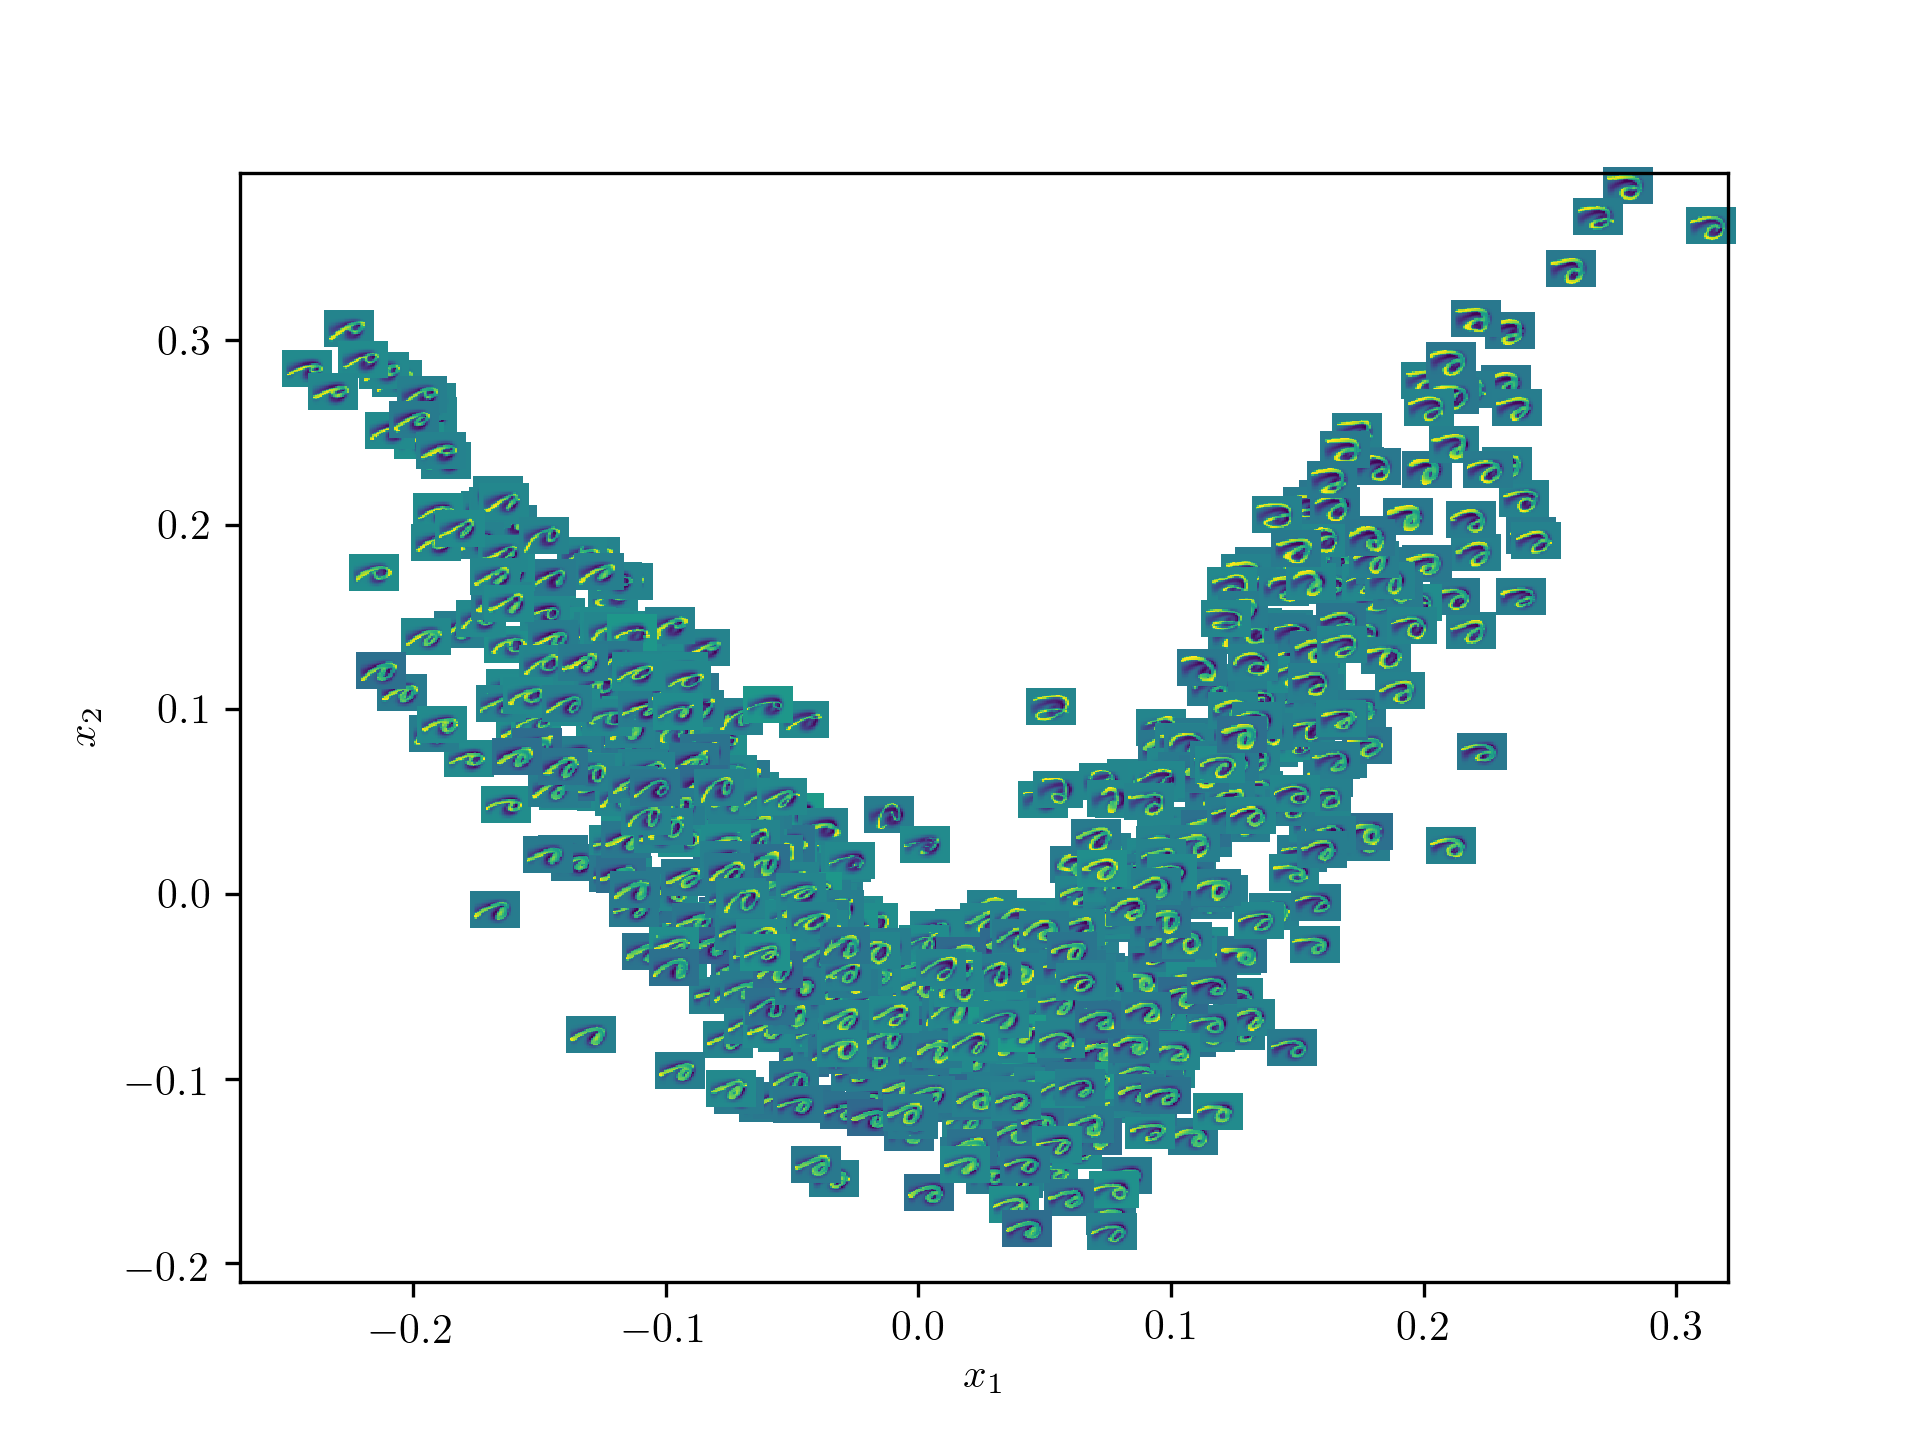
\includegraphics[scale=1.4]{p3/selm_weightspace_images_6.png}}
   \caption{Laplacian Eigenmap Weight Space Scatter Plot}
   \label{fig:leig_scatter}
   \end{figure}
   
   \section{Software Used}
   The following software was used to help in computing the various factorizations:
   
   \begin{itemize}
   \item scikit-learn for ICA, Non-negative Matrix Factorization, and the Laplacian Eigenmap computations
   \end{itemize}
   
   \newpage
   \section{Specialized Software Written}
   
   \begin{minted}[mathescape,
               linenos,
               numbersep=5pt,
               gobble=2,
               frame=lines,
               framesep=2mm]{python}
  # import important libs
  import numpy as np
  import numpy.linalg as la


  def pca( D, k_or_tol ):
     # Author: C. Howard
     # method to perform PCA on some input data given the dimensionality
     # we want our resulting features to have or given a tolerance on the
     # ratio between singular values and the max singular value

     # perform SVD $\ni D = U \Sigma V^{T}$
     [U,S,Vt] = la.svd(D, full_matrices = False )

     # make copy of singular values
     iv = np.copy(S)

     # define current number of weight terms as follow
     k = k_or_tol

     # if we are picking k using a relative difference
     # between singular value magnitudes
     if k_or_tol < 1:
        b = iv >= S[0]*k_or_tol  # find indices $j = 1, \cdots, k \ni \sigma_j$ > $\epsilon$
        k = np.sum(b)

     # compute $W$ and $W^{+}$ using truncated SVD terms
     W       = U[:, :k].T
     Winv    = U[:, :k]

     # return weights and original singular values
     return (W,Winv,S)
\end{minted}

\newpage
\begin{minted}[mathescape,
linenos,
numbersep=5pt,
gobble=2,
frame=lines,
framesep=2mm]{python}
  #import useful libraries
  import numpy as np

  def ica( D , eps = 1e-6, random_seed = 17):
      # Author: C. Howard
      # method to perform ICA using FastICA on some input data to create a set
      # of independent features
      #
      # Inputs:
      #   D           : Dataset where columns represent samples and
      #                 rows are number of dimensions
      #   eps         : the epsilon used to denote when the algorithm has converged
      #   random_seed : seed to use to make algorithm repeatable
      #
      # Outputs:
      #   W   : Mixing Matrix
      #   Winv: Inverse of Mixing Matrix
      #
      # Code based on https://en.wikipedia.org/wiki/FastICA and comments made in
      # Machine Learning a Probabilistic Perspective by Kevin P. Murphy

      # initialize random seed for repeatability
      np.random.seed(seed=random_seed)

      # define the g(u) and g'(u) that will be used
      def g_gderiv(u):
          c = np.tanh(u)
          return (c, 1 - c**2)

      # get number of components that will be used
      (N,M) = D.shape
      ncomp = N

      # define output matrix W
      W = np.random.randn(D.shape[0],ncomp)

      # define some helper entities
      One = np.ones((M,1))

      # compute the components
      for p in range(0,ncomp):

          # set difference between w vectors to arbitrary number above threshold
          dw = 10*eps

          while dw > eps:

              # get current value for vector w
              w0 = np.copy(W[:,p])

              # compute source signal
              z = np.matmul(W[:,p].T,D)

              # compute g and g' given z
              (g,gd) = g_gderiv(z)

              # set the new value for the vector w
              W[:,p] = (np.matmul(D,g.T) - np.matmul(gd,One)*W[:,p])/M

              # orthogonalize relative to the past w components
              if p > 0:
                  W[:,p] = W[:,p] - np.matmul( W[:,:p], (np.matmul(W[:,p].T,W[:,:p])) )

              # normalize to keep on constraint surface
              w1      = W[:,p]
              W[:,p]  = W[:,p]/np.sqrt(np.matmul(W[:,p].T,W[:,p]))
              w2      = W[:,p]

              # compute change in w vector
              dw = np.linalg.norm(w0-W[:,p])

      # Compute inverse of W
      Winv = W.T

      # return W and inverse of W
      return (W,Winv)
\end{minted}


\newpage
\begin{minted}[mathescape,
linenos,
numbersep=5pt,
gobble=2,
frame=lines,
framesep=2mm]{python}
  #import useful libraries
  import numpy as np

  def projrep(A, k_or_tol, random_seed = 17, num_power_method = 4):
    # Author: Christian Howard
    # This function is designed to take some input matrix A
    # and approximate it by the low-rank form A = Q*(Q^T*A) = Q*B.
    # This form is achieved using randomized algorithms and
    # allows for adaptive rank reduction
    #
    # Inputs:
    # A: Matrix to be approximated by low-rank form
    # k_or_tol: If value >= 1, it sets that rank as the target.
    #           If 0 < value < 1, tries to adaptively find low rank form

    # get dimensions of A
    (r, c) = A.shape

    # get the smallest dimension
    sdim = min(r, c)

    if k_or_tol >= 1:
        k = int(k_or_tol)

        # get the random input and measurements from column space
        omega   = np.random.randn(c, k)
        Y       = np.matmul(A, omega)

        # form estimate for Q using power method
        for i in range(1, num_power_method):
            Q1, R1 = np.linalg.qr(Y)
            Q2, R2 = np.linalg.qr(np.matmul(A.T, Q1[:, :k]))
            Y = np.matmul(A, Q2[:, :k])
        Q3, R3 = np.linalg.qr(Y)

        # get final k orthogonal vector estimates from column space
        Q = Q3[:, :k]

        # compute weights associated with the column space to approximate A
        B = np.matmul(Q.T,A)

        # return the two matrices
        return (Q,B)
    else:

        # init some variables used in algorithm
        eps = k_or_tol
        err = 1e20
        kt  = 0
        k   = math.ceil(0.14 * sdim)
        iter_max    = 14
        iter        = 1
        Qt = np.zeros((r, c))

        # adaptively try to estimate the rank via
        # finding column space estimates
        while err > eps and iter_max != iter:

            # get the random input and measurements
            omega = np.random.randn(c, k)
            Y = np.matmul(A, omega)

            # form estimate for Q using power method
            for i in range(1, num_power_method):
                Q1, R1 = np.linalg.qr(Y)
                Q2, R2 = np.linalg.qr(np.matmul(A.T, Q1[:, :k]))
                Y = np.matmul(A, Q2[:, :k])
            Q3, R3 = np.linalg.qr(Y)
            Q = Q3[:, :k]  # get final k orthogonal vector estimates from column space

            # compute error estimate
            o = Q[:, 0]  # use eigenvector from A as initial "random" vec

            # compute normalized eigenvector estimate for error matrix E
            z = np.matmul(A, o)
            y = z - np.matmul(Q, np.matmul(Q.T, z))
            y = y / np.amax(y)

            # use multiple iterations of power method y = (E*E')^{n}*y
            # to get most dominant singular vector
            for i in range(1, num_power_method):
                z = np.matmul(A.T, y)
                y = z - np.matmul(Q, np.matmul(Q.T, z))
                y = y / np.amax(y)
                z = np.matmul(A, y)
                y = z - np.matmul(Q, np.matmul(Q.T, z))
                y = y / np.amax(y)

            # compute largest singular value estimate based on dominant singular vector
            # assume singular value estimate as the error since same as 2-norm of E
            z = np.matmul(A, y)
            err = abs(np.dot(y, z - np.matmul(Q, np.matmul(Q.T, z))) / np.dot(y, y))

            # Stitch new Q vectors to net Q vectors
            Qt[:, kt:(kt + k)] = Q

            # update total k value
            kt = kt + k

            # orthogonalize vectors using QR
            if iter != 1:
                Qh, Rh = np.linalg.qr(Qt[:, :kt])
                Qt[:, :kt] = Qh

            # retreive modified k-recent Q vectors
            Q = Qt[:, (kt - k):kt]

            # compute next best value for k
            # current strategy uses minimized regret method based on solution to
            # the egg drop algorithm problem
            k       = min(sdim, k + math.ceil((iter_max - iter) * sdim / 100.0)) - k
            iter    += 1

            # update matrix A based on new Q vectors
            # Note that new A matrices are essentially error matrices
            # since we subtract approximate projection representations of the kth A matrix
            A = A - np.matmul(Q, np.matmul(Q.T, A))

        # set the final Q matrix
        Q = Qt[:, :kt]

        # compute weights associated with the column space to approximate A
        B = np.matmul(Q.T, A)

        # return the two matrices
        return (Q, B)
\end{minted}
   
   \newpage
   \begin{minted}[mathescape,
linenos,
numbersep=5pt,
gobble=2,
frame=lines,
framesep=2mm]{python}
    #import useful libraries
    import numpy as np
    import math

    def spectrogram(signal, ws = 1024, hs = 512):
        # Author: C. Howard
        # Function to compute the baseline complex valued spectrogram for some sound.
        # signal: a sound represented as a column vector
        # ws    : the window size
        # hs    : the hope size, aka the amount we shift from sample to sample

        # compute Hamming weights
        alpha   = 0.54
        beta    = 1 - alpha
        pi2     = 2.0*math.pi
        c       = pi2/(ws-1)
        w       = alpha - beta * np.cos(c*np.arange(0,ws,1))

        # compute DFT matrix
        p = np.arange(0,ws,1).reshape(ws,1)
        F = np.exp( -(pi2/ws)*np.matmul(p,p.T)*1j )  / np.sqrt(ws)

        # compute resulting local matrix
        D = np.multiply(F,w)

        # Compute number of samples in spectrogram
        (len,c)     = signal.shape
        num_samples = math.floor((len - hs)/(ws - hs))

        # initialize output S
        S = np.zeros((ws,num_samples),dtype=type(F[0,0]))

        # loop through and construct S
        for i in range(0,num_samples):
        S[:ws, i] = np.matmul(D,signal[i*hs:(i*hs+ws),0])

        # return the output spectrogram
        return S[:int(ws/2),:]
\end{minted}
   
\end{document}